\section{Circle sizes}
\label{hdm_circle_size}
A parameter of the Hausdorff distance mask method is the size of the circle mask that is applied on the image. In this section we compare the sizes of 10, 15 and 20 pixels in diameter.

\subsection{Results}

\begin{figure}[H]
    \centering
    \begin{subfigure}{.32\textwidth}
        \centering
        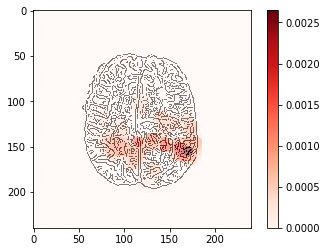
\includegraphics[width=\linewidth]{chapters/06_hdm/b_Brats18_TCIA08_242_1_L2/23.png}
        \caption{T1 modality with pixel mask diameter of 10 pixels}
    \end{subfigure}\hfill%
    \begin{subfigure}{.32\textwidth}
        \centering
        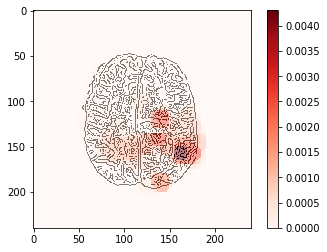
\includegraphics[width=\linewidth]{chapters/06_hdm/circle15/3.png}
        \caption{T1 modality with pixel mask diameter of 15 pixels}
    \end{subfigure}\hfill%
    \begin{subfigure}{.32\textwidth}
        \centering
        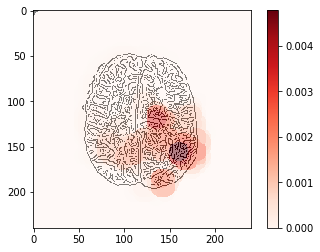
\includegraphics[width=\linewidth]{chapters/06_hdm/circle20/3.png}
        \caption{T1 modality with pixel mask diameter of 20 pixels}
    \end{subfigure}
    \caption{T1 modality HDM results with three different mask diameters.}
    \label{hdm_circle_size_t1}
\end{figure}

\begin{figure}[H]
    \centering
    \begin{subfigure}{.32\textwidth}
        \centering
        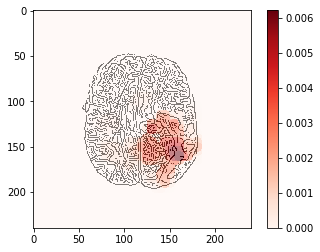
\includegraphics[width=\linewidth]{chapters/06_hdm/b_Brats18_TCIA08_242_1_L2/38.png}
        \caption{FLAIR modality with pixel mask diameter of 10 pixels}
    \end{subfigure}\hfill%
    \begin{subfigure}{.32\textwidth}
        \centering
        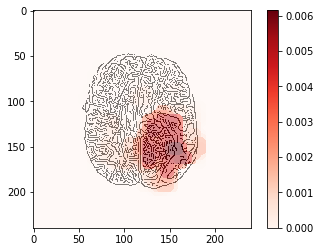
\includegraphics[width=\linewidth]{chapters/06_hdm/circle15/18.png}
        \caption{FLAIR modality with pixel mask diameter of 15 pixels}
    \end{subfigure}\hfill%
    \begin{subfigure}{.32\textwidth}
    \centering
        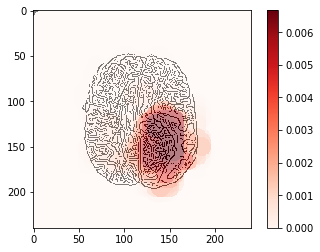
\includegraphics[width=\linewidth]{chapters/06_hdm/circle20/18.png}
        \caption{FLAIR modality with pixel mask diameter of 20 pixels}
    \end{subfigure}
    \caption{FLAIR modality HDM results with three different mask diameters.}
    \label{hdm_circle_size_flair}
\end{figure}

\subsection{Discussion}
Figure \ref{hdm_circle_size_t1} and \ref{hdm_circle_size_flair} show the influence of the mask size when applying Hausdorff distance masks.
Images for the T1 contrast enhanced and T2 modality where also generated, but they look very similar to the FLAIR modality images and therefore omitted here.

\subsection{Conclusion}
The different pixel sizes do not have a big impact on the generated output. A mask diameter of 15 pixels seems to be the optimal case for the BraTS dataset, this diameter
provides enough distinction between circle (compared to 20 pixels, which fills a region completely, removing small distinctions between masks) and also enough
marks enough of the region to have a good insight into the model.
